\documentclass{scrartcl}
        \usepackage{xcolor, tikz}
        \usepackage{pgfplots}
        \pgfplotsset{compat=newest}
        \pagestyle{empty}
        \definecolor{pdg2112}{RGB}{228,26,28}
\definecolor{pdg2212}{RGB}{55,126,184}
\definecolor{pdg1000010020}{RGB}{55,126,184}
\definecolor{pdg1000020040}{RGB}{166,86,40}
\definecolor{pdg11}{RGB}{152,78,163}
\definecolor{pdg12}{RGB}{255,127,0}
\definecolor{pdg22}{RGB}{77,175,74}
\definecolor{pdg1000060120}{RGB}{153,153,153}
\begin{document}
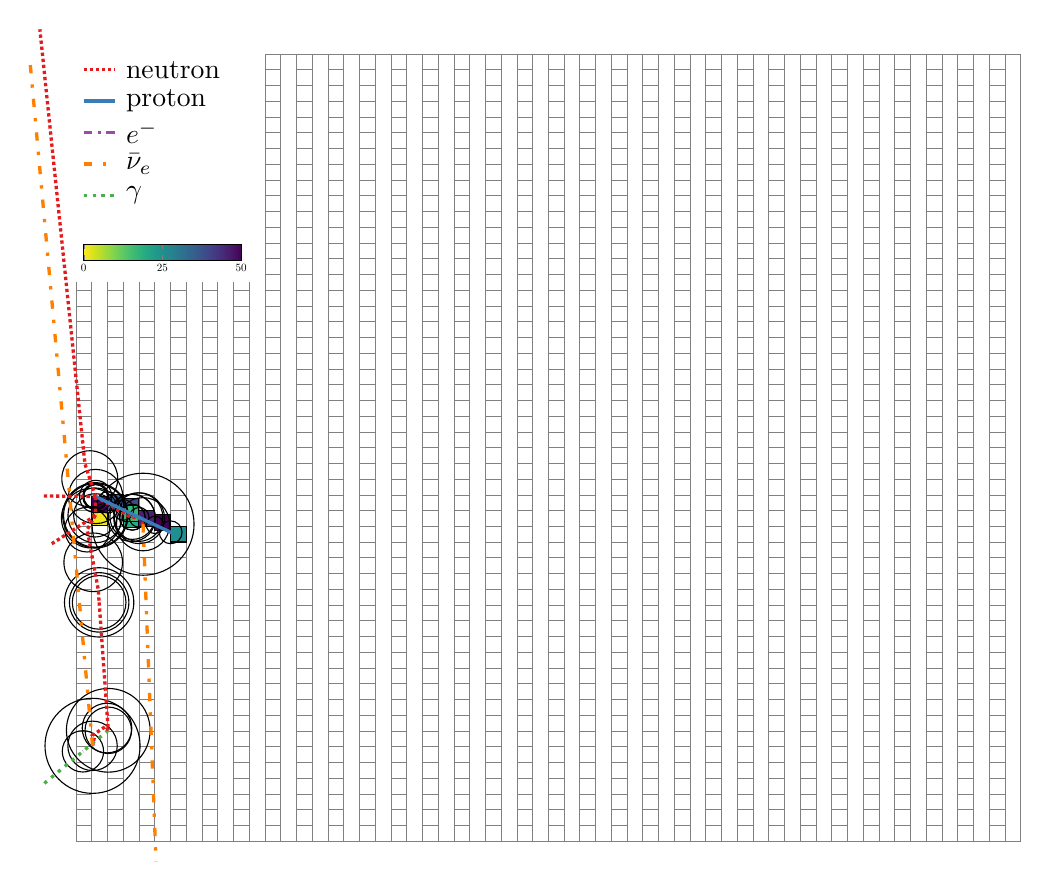
\begin{tikzpicture}[scale=0.4] %\columnwidth/252.0pt]
\draw[step=0.5,very thin,gray] (-0.001000,-12.499) grid (0.500000,5.25);
\draw[step=0.5,very thin,gray] (0.999000,-12.499) grid (1.500000,5.25);
\draw[step=0.5,very thin,gray] (1.999000,-12.499) grid (2.500000,5.25);
\draw[step=0.5,very thin,gray] (2.999000,-12.499) grid (3.500000,5.25);
\draw[step=0.5,very thin,gray] (3.999000,-12.499) grid (4.500000,5.25);
\draw[step=0.5,very thin,gray] (4.999000,-12.499) grid (5.500000,5.25);
\draw[step=0.5,very thin,gray] (5.999000,-12.499) grid (6.500000,12.499);
\draw[step=0.5,very thin,gray] (6.999000,-12.499) grid (7.500000,12.499);
\draw[step=0.5,very thin,gray] (7.999000,-12.499) grid (8.500000,12.499);
\draw[step=0.5,very thin,gray] (8.999000,-12.499) grid (9.500000,12.499);
\draw[step=0.5,very thin,gray] (9.999000,-12.499) grid (10.500000,12.499);
\draw[step=0.5,very thin,gray] (10.999000,-12.499) grid (11.500000,12.499);
\draw[step=0.5,very thin,gray] (11.999000,-12.499) grid (12.500000,12.499);
\draw[step=0.5,very thin,gray] (12.999000,-12.499) grid (13.500000,12.499);
\draw[step=0.5,very thin,gray] (13.999000,-12.499) grid (14.500000,12.499);
\draw[step=0.5,very thin,gray] (14.999000,-12.499) grid (15.500000,12.499);
\draw[step=0.5,very thin,gray] (15.999000,-12.499) grid (16.500000,12.499);
\draw[step=0.5,very thin,gray] (16.999000,-12.499) grid (17.500000,12.499);
\draw[step=0.5,very thin,gray] (17.999000,-12.499) grid (18.500000,12.499);
\draw[step=0.5,very thin,gray] (18.999000,-12.499) grid (19.500000,12.499);
\draw[step=0.5,very thin,gray] (19.999000,-12.499) grid (20.500000,12.499);
\draw[step=0.5,very thin,gray] (20.999000,-12.499) grid (21.500000,12.499);
\draw[step=0.5,very thin,gray] (21.999000,-12.499) grid (22.500000,12.499);
\draw[step=0.5,very thin,gray] (22.999000,-12.499) grid (23.500000,12.499);
\draw[step=0.5,very thin,gray] (23.999000,-12.499) grid (24.500000,12.499);
\draw[step=0.5,very thin,gray] (24.999000,-12.499) grid (25.500000,12.499);
\draw[step=0.5,very thin,gray] (25.999000,-12.499) grid (26.500000,12.499);
\draw[step=0.5,very thin,gray] (26.999000,-12.499) grid (27.500000,12.499);
\draw[step=0.5,very thin,gray] (27.999000,-12.499) grid (28.500000,12.499);
\draw[step=0.5,very thin,gray] (28.999000,-12.499) grid (29.500000,12.499);
\draw[very thin,gray] (0,-12.5) -- (30,-12.5) -- (30,12.5) -- (6,12.5);
\definecolor{tempcolor}{rgb}{0.945636,0.899815,0.112838}\draw[fill=tempcolor,fill opacity=1] (0.500000,-2.471739) rectangle (1.000000,-1.971739);
\definecolor{tempcolor}{rgb}{0.267004,0.004874,0.329415}\draw[fill=tempcolor,fill opacity=1] (0.500000,-2.058944) rectangle (1.000000,-1.558944);
\definecolor{tempcolor}{rgb}{0.218130,0.347432,0.550038}\draw[fill=tempcolor,fill opacity=1] (1.000000,-2.000000) rectangle (1.500000,-1.500000);
\definecolor{tempcolor}{rgb}{0.243113,0.292092,0.538516}\draw[fill=tempcolor,fill opacity=1] (1.500000,-2.118477) rectangle (2.000000,-1.618477);
\definecolor{tempcolor}{rgb}{0.153894,0.680203,0.504172}\draw[fill=tempcolor,fill opacity=1] (1.500000,-2.527900) rectangle (2.000000,-2.027900);
\definecolor{tempcolor}{rgb}{0.202219,0.715272,0.476084}\draw[fill=tempcolor,fill opacity=1] (1.500000,-2.349057) rectangle (2.000000,-1.849057);
\definecolor{tempcolor}{rgb}{0.283072,0.130895,0.449241}\draw[fill=tempcolor,fill opacity=1] (2.000000,-2.500000) rectangle (2.500000,-2.000000);
\definecolor{tempcolor}{rgb}{0.267004,0.004874,0.329415}\draw[fill=tempcolor,fill opacity=1] (2.500000,-2.633721) rectangle (3.000000,-2.133721);
\definecolor{tempcolor}{rgb}{0.129933,0.559582,0.551864}\draw[fill=tempcolor,fill opacity=1] (3.000000,-3.000000) rectangle (3.500000,-2.500000);
\draw (0.628430,-1.554651) circle (-0.861251);
\draw (0.628430,-1.554651) circle (-0.379257);
\draw (0.628430,-1.554651) circle (-0.413480);
\draw (0.628430,-1.554651) circle (-0.512629);
\draw (0.442883,-0.990000) circle (-0.887513);
\draw (2.009998,-2.242968) circle (-0.807411);
\draw (2.133862,-2.434934) circle (-0.844250);
\draw (2.133862,-2.434934) circle (-1.619322);
\draw (1.988965,-2.210365) circle (-0.771382);
\draw (1.795288,-2.219517) circle (-0.404426);
\draw (1.790967,-2.209157) circle (-0.412861);
\draw (1.797241,-2.200432) circle (-0.715828);
\draw (1.777417,-2.234272) circle (-0.749858);
\draw (0.628430,-1.554651) circle (-0.381513);
\draw (1.009998,-1.740545) circle (-0.339646);
\draw (1.509998,-1.980319) circle (-0.329281);
\draw (2.009998,-2.216781) circle (-0.313414);
\draw (2.509998,-2.455047) circle (-0.275267);
\draw (3.009998,-2.692211) circle (-0.362291);
\draw (0.619165,-2.152903) circle (-1.007903);
\draw (0.619165,-2.152903) circle (-0.870146);
\draw (0.619165,-2.152903) circle (-1.037576);
\draw (0.619165,-2.152903) circle (-0.687865);
\draw (0.490002,-2.241757) circle (-0.946708);
\draw (0.551392,-3.643953) circle (-0.929519);
\draw (0.740405,-4.916166) circle (-0.852002);
\draw (0.740405,-4.916166) circle (-1.100519);
\draw (0.740405,-4.916166) circle (-0.943314);
\draw (1.029578,-8.977827) circle (-1.328822);
\draw (0.225403,-9.646256) circle (-0.655940);
\draw (1.029578,-8.977827) circle (-0.737151);
\draw (0.990002,-8.906839) circle (-0.787372);
\draw (0.530029,-9.470839) circle (-0.784359);
\draw (0.530029,-9.470839) circle (-1.509270);
\draw (0.359717,-2.607590) circle (-0.708753);
\draw[color=pdg2112, very thick, densely dotted] (-1.0147461997320988, -1.537691322296926) -- (-0.014845167515522917, -1.548011398285496) -- (0.0029999999999745343, -1.548195579998341) -- (0.48999999999998634, -1.5532219544539132) -- (0.6284312103700586, -1.554650716465531);
\draw[color=pdg1000020040, very thick, solid] (0.6284312103700586, -1.554650716465531);
\draw[color=pdg2212, very thick, solid] (0.6284312103700586, -1.554650716465531) -- (0.6224548484315392, -1.5331535778418757) -- (0.6178103757242752, -1.516010050545358) -- (0.6141089523766141, -1.5022653147460647) -- (0.6109005187039657, -1.4912743872518404);
\draw[color=pdg1000010020, very thick, solid] (0.6284312103700586, -1.554650716465531) -- (0.6275731653993943, -1.5428046653475485);
\draw[color=pdg2212, very thick, solid] (0.6284312103700586, -1.554650716465531);
\draw[color=pdg2112, very thick, densely dotted] (0.6284312103700586, -1.554650716465531) -- (0.5860371408537048, -1.4256396876143307) -- (0.5800574189430335, -1.4074425651219213) -- (0.574931943019601, -1.3918450315569992) -- (0.5706607130833845, -1.378847086919564) -- (0.5100000000000137, -1.1942481301547567) -- (0.5029999999999972, -1.1729461600381477) -- (0.4970000000000027, -1.1546873285096486) -- (0.49200000000000726, -1.139471635569218) -- (0.4494545713835805, -1.0100000000000002) -- (0.28956088948762043, -0.5234213666314071) -- (0.2881684851957516, -0.51) -- (0.23629581342884193, -0.009999999999999929) -- (0.18442314166190954, 0.4900000000000001) -- (0.13255046989497715, 0.99) -- (0.08067779812806748, 1.49) -- (0.02880512636113508, 1.9900000000000002) -- (0.010000000000013642, 2.171262365332142) -- (0.007999999999992725, 2.190540338992285) -- (0.003000000000020009, 2.2387352731423262) -- (-0.08509887014461129, 3.087919122207349) -- (-0.17319774028926532, 3.9371029712723717) -- (-0.2612966104338966, 4.786286820337394) -- (-0.34939548057855063, 5.635470669402417) -- (-0.43749435072318194, 6.48465451846744) -- (-0.5255932208678132, 7.333838367532462) -- (-0.6136920910124672, 8.183022216597486) -- (-0.7017909611570985, 9.032206065662509) -- (-0.7898898313017526, 9.881389914727531) -- (-0.8779887014463839, 10.730573763792554) -- (-0.9660875715910151, 11.579757612857577) -- (-1.0541864417356692, 12.428941461922602) -- (-1.1422853118803005, 13.278125310987624);
\draw[color=pdg2112, very thick, densely dotted] (0.6284312103700586, -1.554650716465531) -- (0.7620892454834575, -1.6337091451208419) -- (0.9173710382017817, -1.7255579780075336) -- (0.9900000000000091, -1.768517846374324) -- (0.9970000000000254, -1.7726583307089783) -- (1.0029999999999972, -1.7762073172815274) -- (1.0080000000000156, -1.7791648060920007) -- (1.364442927462619, -1.9899999999999998) -- (1.3678241744058368, -1.9920000000000002) -- (1.3762772917639041, -1.9969999999999999) -- (1.3864210325935573, -2.0029999999999997) -- (1.3948741499516246, -2.008) -- (1.3982553968948424, -2.01) -- (1.490000000000009, -2.064266727420815) -- (1.4970000000000254, -2.0684072117554693) -- (1.5029999999999972, -2.071956198328018) -- (1.5080000000000156, -2.0749136871384914) -- (1.538498209075192, -2.092953309554303) -- (1.6937800017935387, -2.184802142440995) -- (1.7774149688112857, -2.2342720382647148) -- (1.795289713696866, -2.2195171732371266) -- (1.9889626816173631, -2.210364580634505) -- (1.9970000000000028, -2.222820763594039) -- (2.0029999999999974, -2.23211952397645) -- (2.007999999999993, -2.239868490961802) -- (2.1338657880329266, -2.4349344581719676);
\draw[color=pdg11, very thick, dashdotted] (2.1338657880329266, -2.4349344581719676);
\draw[color=pdg12, very thick, loosely dashdotted] (2.1338657880329266, -2.4349344581719676) -- (2.1359896775070184, -2.49) -- (2.1552747821620644, -2.99) -- (2.17455988681711, -3.4899999999999998) -- (2.193844991472156, -3.9900000000000007) -- (2.213130096127202, -4.49) -- (2.2324152007822478, -4.99) -- (2.2517003054372937, -5.49) -- (2.2709854100923392, -5.99) -- (2.290270514747385, -6.49) -- (2.309555619402431, -6.989999999999999) -- (2.328840724057477, -7.489999999999999) -- (2.348125828712523, -7.989999999999999) -- (2.3674109333675686, -8.489999999999998) -- (2.3866960380226145, -8.989999999999998) -- (2.4059811426776605, -9.489999999999998) -- (2.4252662473327065, -9.989999999999998) -- (2.4445513519877524, -10.49) -- (2.463836456642798, -10.99) -- (2.483121561297844, -11.49) -- (2.490000000000009, -11.668335529549616) -- (2.492000000000007, -11.720189020514937) -- (2.4970000000000026, -11.849822747928688) -- (2.5029999999999974, -12.005383220825356) -- (2.507999999999993, -12.135016948239372) -- (2.5100000000000136, -12.186870439205116) -- (2.5135280399868636, -12.278341033997318) -- (2.5331715370885832, -12.787632983745912) -- (2.5336523318972013, -12.800098428378282) -- (2.544657178013222, -13.085418272705542) -- (2.5474333493359156, -13.157395360006257);
\draw[color=pdg2212, very thick, solid] (2.1338657880329266, -2.4349344581719676);
\draw[color=pdg2212, very thick, solid] (1.9889626816173631, -2.210364580634505);
\draw[color=pdg2212, very thick, solid] (1.795289713696866, -2.2195171732371266) -- (1.795140616807157, -2.21252082580519) -- (1.7953663778518603, -2.2065633586937192) -- (1.7962843870495135, -2.2024581218329553) -- (1.7972423728944478, -2.2004322380410883) -- (1.787454179202291, -2.214692096356079) -- (1.7847926433827752, -2.2192733862082146);
\draw[color=pdg1000060120, very thick, loosely dashdotted] (1.7972423728944478, -2.2004322380410883);
\draw[color=pdg1000060120, very thick, loosely dashdotted] (1.7774149688112857, -2.2342720382647148);
\draw[color=pdg1000010020, very thick, solid] (0.6284312103700586, -1.554650716465531) -- (0.9900000000000091, -1.7309244652521794) -- (1.4318619140341298, -1.9434136760223182) -- (1.490000000000009, -1.970957922907941) -- (1.8302372863041683, -2.1306742500870506) -- (1.990000000000009, -2.207211759737002) -- (2.2280464267731075, -2.3216682658722476) -- (2.40425181672972, -2.406055811497813) -- (2.490000000000009, -2.445701404461971) -- (2.630344681578572, -2.511303126308553) -- (2.7264283427432927, -2.556457659561919) -- (2.802638954068789, -2.5921055474469394) -- (2.863176727084851, -2.6215409798690046) -- (2.9119546115481625, -2.6449630247214317) -- (2.951322354205786, -2.6637363696223124) -- (2.9827158746875737, -2.6790264541307103) -- (3.0302537269560617, -2.7017824284148757) -- (3.046518572943296, -2.7093855780167027) -- (3.0596288096016453, -2.715296537328327) -- (3.070127306584891, -2.7200211169041126);
\draw[color=pdg2112, very thick, densely dotted] (0.6284312103700586, -1.554650716465531) -- (0.6274114101999885, -1.62045627849247) -- (0.6191599981000764, -2.1529025622777858);
\draw[color=pdg1000020040, very thick, solid] (0.6191599981000764, -2.1529025622777858);
\draw[color=pdg1000010020, very thick, solid] (0.6191599981000764, -2.1529025622777858);
\draw[color=pdg1000020040, very thick, solid] (0.6191599981000764, -2.1529025622777858);
\draw[color=pdg2212, very thick, solid] (0.6191599981000764, -2.1529025622777858);
\draw[color=pdg2112, very thick, densely dotted] (0.6191599981000764, -2.1529025622777858) -- (0.5100000000000137, -2.22799857632753) -- (0.35436317285500535, -2.3350680666294887) -- (0.1139418108325799, -2.4899999999999998) -- (0.09376857967035904, -2.503) -- (0.009999999999990905, -2.556982008482348) -- (-0.8139864379904793, -3.0879739753984627);
\draw[color=pdg2112, very thick, densely dotted] (0.6191599981000764, -2.1529025622777858) -- (0.5745800403191424, -2.231031199343376) -- (0.5100000000000137, -2.344210995442917) -- (0.5029999999999972, -2.3564788504764915) -- (0.4970000000000027, -2.3669941547909694) -- (0.49200000000000726, -2.3757569083863763) -- (0.42681324656123254, -2.4899999999999998) -- (0.4193954869161189, -2.503) -- (0.359716530763626, -2.607590397519006) -- (0.43044247040838857, -2.99) -- (0.4900000000000091, -3.3120228862319285) -- (0.49200000000000726, -3.3228367291981753) -- (0.4970000000000027, -3.349871336613871) -- (0.5029999999999972, -3.3823128655127377) -- (0.5079999999999927, -3.409347472928487) -- (0.5100000000000137, -3.4201613158948234) -- (0.5443620860706005, -3.605954417275614) -- (0.5468217863185145, -3.619253823388103) -- (0.5489301008167103, -3.6306533143416657) -- (0.5506870295652334, -3.6401528901363016) -- (0.7086667457906287, -4.494336811696769) -- (0.7168627415409674, -4.603259323816031) -- (0.7186329656321278, -4.626785111395392) -- (0.7201503005674113, -4.646950072177704) -- (0.721414746346818, -4.66375420616296) -- (0.7404077265729029, -4.916165649735168);
\draw[color=pdg1000020040, very thick, solid] (0.7404077265729029, -4.916165649735168);
\draw[color=pdg1000020040, very thick, solid] (0.7404077265729029, -4.916165649735168);
\draw[color=pdg1000020040, very thick, solid] (0.7404077265729029, -4.916165649735168);
\draw[color=pdg2112, very thick, densely dotted] (0.7404077265729029, -4.916165649735168) -- (0.7687662209041491, -5.314481738806682) -- (0.8036135681616543, -5.803938580626391) -- (0.8384609154191821, -6.2933954224461015) -- (0.8733082626766873, -6.782852264265811) -- (0.9081556099341924, -7.27230910608552) -- (0.9430029571916976, -7.761765947905228) -- (0.9778503044492026, -8.251222789724938) -- (0.9899999999999863, -8.42187427631939) -- (0.9920000000000073, -8.449965759909514) -- (0.99699999999998, -8.520194468884307) -- (1.0029999999999972, -8.60446891965447) -- (1.0079999999999927, -8.674697628629405) -- (1.0100000000000136, -8.70278911221944) -- (1.029581617214376, -8.977827451540675);
\draw[color=pdg22, very thick, dotted] (1.029581617214376, -8.977827451540675);
\draw[color=pdg22, very thick, dotted] (1.029581617214376, -8.977827451540675) -- (1.014936996023539, -8.99) -- (1.0065153948544547, -8.997) -- (0.9970000000000028, -9.004909156779553) -- (0.9920000000000073, -9.00906513606393) -- (0.9596683888272082, -9.035939037316844) -- (0.8023876087451753, -9.166670170087059) -- (0.6451068286631653, -9.297401302857272) -- (0.5100000000000137, -9.409701539077588) -- (0.5029999999999972, -9.41551991007572) -- (0.4970000000000027, -9.420507085216968) -- (0.49200000000000726, -9.424663064501345) -- (0.41339405537426044, -9.489999999999998) -- (0.4049724542051763, -9.497) -- (0.39775393891738986, -9.503) -- (0.39173850951090117, -9.508) -- (0.225404534123777, -9.646256111199307) -- (0.010000000000013642, -9.824816334772795) -- (-0.5059872299084418, -10.252545470133406) -- (-1.0149744598168808, -10.674471934858046);
\draw[color=pdg11, very thick, dashdotted] (0.225404534123777, -9.646256111199307) -- (0.22850805332482196, -9.643721487960317);
\draw[color=pdg1000060120, very thick, loosely dashdotted] (1.029581617214376, -8.977827451540675);
\draw[color=pdg2112, very thick, densely dotted] (1.029581617214376, -8.977827451540675) -- (1.0100000000000136, -8.942708345645785) -- (1.00300000000002, -8.930154033171343) -- (0.9970000000000028, -8.919393193907505) -- (0.9920000000000073, -8.910425827854331) -- (0.9565307019293414, -8.846812591964591) -- (0.527894420162579, -9.13834561407172) -- (0.5520821754540293, -9.16660393679686) -- (0.5893677997039959, -9.200476766430024) -- (0.5300238698196835, -9.470838638848958);
\draw[color=pdg11, very thick, dashdotted] (0.5300238698196835, -9.470838638848958);
\draw[color=pdg12, very thick, loosely dashdotted] (0.5300238698196835, -9.470838638848958) -- (0.5208877655452853, -9.370875411478824) -- (0.5189321518518681, -9.349477948138759) -- (0.5099999999999909, -9.251746278309353) -- (0.5079999999999927, -9.22986315956037) -- (0.5029999999999972, -9.175155362687835) -- (0.4970000000000027, -9.109506006440741) -- (0.49200000000000726, -9.054798209568096) -- (0.48999999999998634, -9.032915090818934) -- (0.48790568327285655, -9.010000000000002) -- (0.44220835779246953, -8.510000000000002) -- (0.3965110323120825, -8.010000000000002) -- (0.3508137068316728, -7.510000000000001) -- (0.30511638135128577, -7.010000000000001) -- (0.25941905587087605, -6.510000000000001) -- (0.21372173039048903, -6.01) -- (0.168024404910102, -5.51) -- (0.12232707942969227, -5.01) -- (0.07662975394930527, -4.51) -- (0.030932428468895524, -4.01) -- (0.009999999999990905, -3.780966591054743) -- (0.007999999999992725, -3.75908347230576) -- (0.0029999999999972713, -3.704375675433225) -- (-0.07487175539747568, -2.852337240154225) -- (-0.15274351079497137, -2.0002988048752246) -- (-0.23061526619244432, -1.1482603695962248) -- (-0.30848702158991725, -0.2962219343172248) -- (-0.38635877698741294, 0.5558165009617752) -- (-0.46423053238488593, 1.407854936240775) -- (-0.5421022877823816, 2.2598933715197753) -- (-0.6199740431798546, 3.111931806798775) -- (-0.6978457985773275, 3.9639702420777754) -- (-0.7757175539748232, 4.816008677356775) -- (-0.8535893093722962, 5.668047112635775) -- (-0.9314610647697918, 6.520085547914775) -- (-1.0093328201672649, 7.372123983193774) -- (-1.0872045755647377, 8.224162418472774) -- (-1.1650763309622334, 9.076200853751773) -- (-1.2429480863597064, 9.928239289030774) -- (-1.3208198417572021, 10.780277724309773) -- (-1.398691597154675, 11.632316159588772) -- (-1.476563352552148, 12.484354594867773);
\draw[color=pdg2212, very thick, solid] (0.5300238698196835, -9.470838638848958);
\draw[color=pdg1000060120, very thick, loosely dashdotted] (0.359716530763626, -2.607590397519006);
\draw[color=pdg2112, very thick, densely dotted] (0.25,12) -- (1.25,12) node [right,black] {neutron};
\draw[color=pdg2212, very thick, solid] (0.25,11) -- (1.25,11) node [right,black] {proton};
\draw[color=pdg11, very thick, dashdotted] (0.25,10) -- (1.25,10) node [right,black] {$e^-$};
\draw[color=pdg12, very thick, loosely dashdotted] (0.25,9) -- (1.25,9) node [right,black] {$\bar{\nu}_e$};
\draw[color=pdg22, very thick, dotted] (0.25,8) -- (1.25,8) node [right,black] {$\gamma$};

        \begin{axis}[%
            at={(0.25cm,6.75cm)},
            hide axis,
            scale only axis,
            height=0pt,
            width=0pt,
            colormap={reverse viridis}{
                indices of colormap={
                \pgfplotscolormaplastindexof{viridis},...,0 of viridis}
            },
            colorbar horizontal,
            point meta min=0,
            point meta max=50,
            colorbar style={
                width=5cm,
                xtick={50, 25, 0},
            }]
            %\addplot [draw=none] coordinates {(1,15)};
        \end{axis}
        
        \end{tikzpicture}
        \end{document}
        